%%%%%%%%%%%%%%%%%%%%%%%%%%%%%%%%%%%%%%%%%
% Beamer Presentation
% LaTeX Template
% Version 1.0 (10/11/12)
%
% This template has been downloaded from:
% http://www.LaTeXTemplates.com
%
% License:
% CC BY-NC-SA 3.0 (http://creativecommons.org/licenses/by-nc-sa/3.0/)
%
%%%%%%%%%%%%%%%%%%%%%%%%%%%%%%%%%%%%%%%%%

%----------------------------------------------------------------------------------------
%	PACKAGES AND THEMES
%----------------------------------------------------------------------------------------

\documentclass{beamer}

\newcommand\mybeamerex[2]{%
  \newtheorem*{#1}{#2}%
  \AtBeginEnvironment{#1}{%
     \setbeamercolor{block body}{fg=black,bg=green!5}%
     \setbeamercolor{block title}{fg=white,bg=green!65!black}%
  }%
}

\mode<presentation> {

% The Beamer class comes with a number of default slide themes
% which change the colors and layouts of slides. Below this is a list
% of all the themes, uncomment each in turn to see what they look like.

%\usetheme{default}
%\usetheme{AnnArbor} %no
%\usetheme{Antibes}
%\usetheme{Bergen} %no
%\usetheme{Berkeley} %no
%\usetheme{Berlin}
%\usetheme{Boadilla}
%\usetheme{CambridgeUS}
%\usetheme{Copenhagen}
%\usetheme{Darmstadt}
%\usetheme{Dresden}
%\usetheme{Frankfurt}
%\usetheme{Goettingen}
%\usetheme{Hannover}
%\usetheme{Ilmenau}
%\usetheme{JuanLesPins}
%\usetheme{Luebeck}
%\usetheme{Madrid}
%\usetheme{Malmoe}
%\usetheme{Marburg}
\usetheme{Montpellier}
%\usetheme{PaloAlto}
%\usetheme{Pittsburgh}
%\usetheme{Rochester}
%\usetheme{Singapore}
%\usetheme{Szeged}
%\usetheme{Warsaw}

% As well as themes, the Beamer class has a number of color themes
% for any slide theme. Uncomment each of these in turn to see how it
% changes the colors of your current slide theme.

%\usecolortheme{albatross}
%\usecolortheme{beaver}
%\usecolortheme{beetle}
%\usecolortheme{crane}
\usecolortheme{dolphin}
%\usecolortheme{dove}
%\usecolortheme{fly}
%\usecolortheme{lily}
%\usecolortheme{orchid}
%\usecolortheme{rose}
%\usecolortheme{seagull}
%\usecolortheme{seahorse}
%\usecolortheme{whale}
%\usecolortheme{wolverine}

%\setbeamertemplate{footline} % To remove the footer line in all slides uncomment this line
%\setbeamertemplate{footline}[page number] % To replace the footer line in all slides with a simple slide count uncomment this line

%\setbeamertemplate{navigation symbols}{} % To remove the navigation symbols from the bottom of all slides uncomment this line
}

\usepackage{graphicx} % Allows including images
\usepackage{booktabs} % Allows the use of \toprule, \midrule and \bottomrule in tables
\usepackage{tikz}

\usepackage{wrapfig}

\usepackage{pgfplots}

\definecolor{light-gray}{gray}{0.8}

\usepackage{scalefnt}
\usepackage{etoolbox}
\usepackage{ragged2e}

\apptocmd{\frame}{}{\justifying}{} % Allow optional arguments after frame.


%----------------------------------------------------------------------------------------
%	TITLE PAGE
%----------------------------------------------------------------------------------------

\title{An xgboost solution for Actuarial Loss Prediction} % The short title appears at the bottom of every slide, the full title is only on the title page

\author{A. Guly\'{a}s \& N. Fornasin} % Your name
\institute[ALU] % Your institution as it will appear on the bottom of every slide, may be shorthand to save space
{
Team Boosted Goose\\ % Your institution for the title page
\medskip
%\textit{john@smith.com} % Your email address
}
\date{\quad} % Date, can be changed to a custom date

\begin{document}

\begin{frame}
\titlepage % Print the title page as the first slide
\end{frame}

%\begin{frame}
%\frametitle{The $a$ invariant under cone-edge degeneration} % Table of contents slide, comment this block out to remove it
%\tableofcontents % Throughout your presentation, if you choose to use \section{} and \subsection{} commands, these will automatically be printed on this slide as an overview of your presentation
%\end{frame}

%----------------------------------------------------------------------------------------
%	PRESENTATION SLIDES
%----------------------------------------------------------------------------------------

%------------------------------------------------
%\section{Introduction} % Sections can be created in order to organize your presentation into discrete blocks, all sections and subsections are automatically printed in the table of contents as an overview of the talk
%------------------------------------------------


%------------------------------------------------

\section{Preprocessing}
%\subsection*{The $a$ invariant}
\begin{frame}
\frametitle{Preprocessing}
We used pandas because sklearn's pipelines have been designed with the intention of making me angry (it worked). What we did in preprocessing
\begin{itemize}
\item Corrected mistakes, such as: 200 hours worked per week, reporting date before accident date...
\item Added features, such as: weekday of accident, core working hours, numeric transformations.
\end{itemize}
It wasn't fancy but it did what it had to, which is more than you can ask.
\end{frame}

%------------------------------------------------

\section{Text analysis}
\begin{frame}
\frametitle{Text analysis}
\emph{Try to classify sentences based on word occurrence. Weight clusters of words based on median ultimate.}


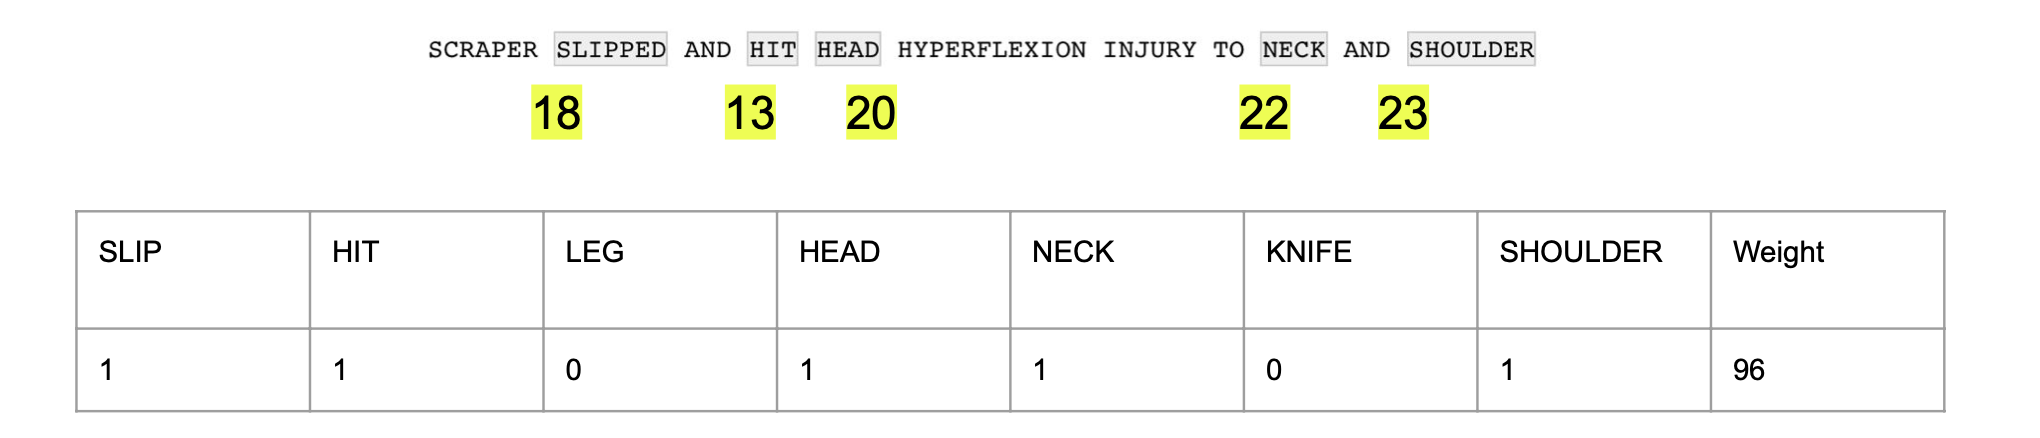
\includegraphics[width=\textwidth]{./images/claimdescription.png}
\end{frame}

%------------------------------------------------

\section{ML Algorithm}
\begin{frame}
\frametitle{ML Algorithm}
After several attempts we decided to focus on a gradient boosted tree. \emph{Write something about ensemble techniques and the number of parallel trees and all these things.}
\end{frame}

%------------------------------------------------

\section{Conclusions}
\begin{frame}
\frametitle{What worked and what didn't}
%\begin{columns}
%	\begin{column}{0.5\textwidth}
 	  	\begin{exampleblock}{\begin{center}What worked\end{center}}
			\justifying
			\begin{itemize}
  				\item Single word analysis;
 				\item Regression to distribution;
  				\item \emph{Stacking with expert judgement (cooking).}
  			\end{itemize}
		\end{exampleblock}
%	\end{column}
%	\begin{column}{0.5\textwidth}  
		\begin{alertblock}{\begin{center}What didn't work\end{center}}
			\begin{itemize}
  				\item Neural networks;
 				\item External data sources (e.g. for inflation);
  				\item \emph{Something about NLP? Like with entity analysis?}
  			\end{itemize}
		\end{alertblock}
%	\end{column}
%\end{columns}
\end{frame}

%----------------------------------------------------------------------------------------

\end{document} 